%%%%%%%%%%%%%%%%%%%%%%%%%%%%%%%%%%%%%%%%%%%%%%%%%%%
%
%  New template code for TAMU Theses and Dissertations starting Fall 2012.  
%  For more info about this template or the 
%  TAMU LaTeX User's Group, see http://www.howdy.me/.
%
%  Author: Wendy Lynn Turner 
%	 Version 1.0 
%  Last updated 8/5/2012
%
%%%%%%%%%%%%%%%%%%%%%%%%%%%%%%%%%%%%%%%%%%%%%%%%%%%
%%%%%%%%%%%%%%%%%%%%%%%%%%%%%%%%%%%%%%%%%%%%%%%%%%%%%%%%%%%%%%%%%%%%%%
%%                           SECTION III
%%%%%%%%%%%%%%%%%%%%%%%%%%%%%%%%%%%%%%%%%%%%%%%%%%%%%%%%%%%%%%%%%%%%%



\chapter{\uppercase{Optimization Methodology}}

In order to optimize the system, the energy use from each of the components comprising the air-side equipment needs to be estimated. This includes fan energy, cooling energy, and reheat energy.


Fan Energy:
\begin{equation} \label{eq:FanEqnergy} 
\dot E_{fan} = fct\left( {\flow{supply},\Delta {P_{s,{\rm{fan}}}}} \right)
\end{equation}

Cooling Energy:
\begin{equation} \label{eq:CoolingEnergy}
{\dot E_{cooling}} = {\dot V_{{\rm{supply}}}}\rho_a c_{p,a}\:\left( {{T_{ma}} - {\sat}} \right) + h_v\rho_a{\dot V_{{\rm{supply}}}}\:\left( {{\omega _{ma}} - {\omega _{sa}}} \right)
\end{equation}

\section{Reheat in Terminal Units}

Terminal Boxes can be distributed into 3 classifications for this work. Terminal units with no fans, series flow, or parallel flow arrangements.

\subsection{No Fan in Terminal Unit}

If there is no fan and only a damper for air volume modulation, then the reheat energy use is 

\begin{equation} \label{eq:ReheatEnergy}
{\dot E_{reheat}} = \sum\limits_i {{{\dot V}_i}\rho_a c_{p,a}\:\left( {{T_{i,dis}} - {T_{i,sa}}} \right)} 
\end{equation}

\subsection{Series Flow Configuration}

For a series flow terminal unit, the total flow is ideally constant. \(\dot V_{tot}\) is known from specification of the terminal unit and   \({\dot V_{pri}}\) is a measured variable. \(\dot V_{plen}\) can be calculated from Eq. (\ref{eq:TotalFlow}). 

%-------------------------------------------------------------------------------------------
\begin{figure}
\centering
\begin{tikzpicture}
\begin{axis}[
	xmin=0,
    xmax=100,
    ymin=0,
    ymax=120,
	grid=major, 
	ylabel = {Percent Design CFM},
	%height=9cm,
    xtick=\empty, 
    ytick={0,25,...,100},
    ymajorgrids=false,
    clip mode=individual,
]
\addplot[
	no markers, 
	mark=o,
    color=black,
    dashed,
] 
table[x=RoomConditionsPrimary,y=PercentDesignCFMPrimary,col sep=tab] {SeriesFanPlot.dat};

\addplot[
	no markers,
    color=black,
    solid,
]
table[x=RoomConditionsTotal,y=PercentDesignCFMTotal,col sep=tab]{SeriesFanPlot.dat};


\node at (25,60) {Plenum Air};
\node at (78,20) {Primary Air};
\node at (50,110) {Total Air};
\node [anchor=south west] at (0, -15) {Heating};
\node [anchor=south east] at (100, -15) {Cooling};

\end{axis}
\end{tikzpicture}
\begin{tikzpicture}
\begin{axis}[
	xmin=0,
    xmax=100,
    ymin=50,
    ymax=110,
	grid=major, 
	ylabel = {Discharge Air Temperature \(^\circ\)F},
	%height=9cm,
    xtick=\empty, 
    ytick={50,60,...,100},
    ymajorgrids=false,
    clip = false,
    clip mode=individual,
]
\addplot[
	no markers,
    color=black,
    solid,
]
table[x=RoomTemp,y=Tdischarge,col sep=tab]{SeriesFanPlot.dat};
\node [anchor=south west] at (0, -60) {Heating};
\node [anchor=south east] at (100, -60
) {Cooling};
\end{axis}
\end{tikzpicture}
\caption{Example Series Terminal Unit Flow Operation.}
\label{fig:SeriesFlow}

\end{figure}
%-------------------------------------------------------------------------------------------


\begin{equation} \label{eq:TotalFlow}
{\dot V_{plenum}} = {\dot V_{tot}} - {\dot V_{pri}}
\end{equation}

\(T_{dis}\) will be sensed. The temperature of the air after mixing can be estimated from the flow information and an assumption or measurement of plenum air. 


\begin{equation} \label{eq:MixedAirTemperature}
{T_{mix}} = \frac{{{{\dot V}_{pri}}\left( {{T_{pri}}} \right) + \dot V_{plen}\left( {{T_{plen}}} \right)}}{{{{\dot V}_{total}}}}
\end{equation}




The increase in temperature to the discharge temperature is due to heat gain from the fan and from any supplementary heating.

The temperature rise from the fan, \(\Delta T_{fan}\), can be estimated from historical data when the supplementary heating is off, either when the heating coil is completely closed or all stages of electrical reheat are inactive. If there is no other heating, the temperature increase from the fan is

\begin{equation}
\Delta {T_{fan}} = {T_{dis}} - {T_{mix}}.
\end{equation}
%
For other times, the temperature increase due to reheat will be
%
\begin{equation}
\Delta {T_{reheat}} = {T_{dis}} - \left( {\Delta {T_{fan}} + {T_{mix}}} \right),
\end{equation}
%
and the reheat energy will be
%
\begin{equation}
{\dot Q_{reheat}} = {\dot V_{tot}}{\rho _a}{c_{p,a}}\left( {\Delta {T_{reheat}}} \right).
\end{equation}

\subsection{Parallel Flow Configuration}

During periods of cooling, the fan in a parallel arrangement is off and the total flow is equal to the primary flow.

The fan volume flow will be known from manufacturers specifications and the total flow can be calculated using Eq. \eqref{eq:TotalFlow}. The temperature from mixing the plenum air and primary can be estimated from Eq. \eqref{eq:MixedAirTemperature} or from historical data when the primary flow is at the minimum and there is no activated reheat components.

\subsection{Other Terminal Unit Types}

Terminal units come in even more configurations than the three specified in this document, induction units being one example. Using a combination of energy balances, historical data under particular conditions, and appropriate assumptions, a model of the terminal unit can be made. 

\section{Required Sensors}

In order to fulfill the proposed methodology, there are several sensors that are not common that would need to be installed. 

Table \ref{tab:NecessarySensors} lists the minimum set of sensors required. The sensors that are least likely to be available are the static pressure at the fan and the discharge air temperature from each terminal box.

\begin{table}
\centering
\begin{tabular}{l l}
\toprule

Level & Sensor \\
\midrule\midrule
\multirow{2}{*}{Weather} & Outdoor Air Temperature \\
 & Outdoor Dew Point Temperature \\
 
 \midrule
 
 \multirow{6}{*}{AHU} & Supply Air Temperature \\
 & Mixed Air Temperature \\
 & Fan Power \\
 & VFD Command \\
 & Static Pressure at Fan \\
 & Static Pressure for Control \\
 
 
\midrule
\multirow{4}{*}{Terminal Units} & Primary Air Flow Rate \\
& Discharge Air Temperature \\
& Primary Damper Position \\

\bottomrule

\end{tabular}
\caption{Necessary Sensors}
\label{tab:NecessarySensors}
\end{table}

\section{Predicting Zone Loads}

The zone loads can be estimated from terminal unit data of airflow rate, terminal unit leaving temperature and zone temperature. Note that using 

\begin{equation}
\dot Q_{zone} = \dot V_{zone} C_{air} \left(T_{zone}-T_{leaving} \right)
\end{equation}

assumes that the space is well-mixed and at steady-state. If the controls oscillate, then the zone load estimation will have some periodicity. In one sense, there is no ``single'' zone load coming from a point source, and as such we will have to use only an estimation.

The independent variables available for prediction are the current time and outdoor air conditions. The current time can be separated into time of day, day of week, weekdays/weekends and such. Outdoor air temperature correlates with the external load. 

The approach used is a related to the concept of a \textit{nearest neighbor}. The nearest neighbors are defined by any previous data that:

\begin{enumerate}
\item Was within 1 hour of the time of day 
\item Was the same day of the week
\item Had a corresponding \(T_{db}\) that is within \(\pm 2.5^\circ\)F of the the current \(T_{db}\). 
\end{enumerate}

The median value of the nearest neighbors can be used to estimate the particular zone load at any time and temperature.  The median is a more robust statistic in comparison to the mean, having a breakdown point of 50\%, meaning that up to 50\% of the data can be contaminated before the median statistic will no longer be reliable. For the mean, one arbitralily large data point can turn the mean statistic unreliable. 

It is advised that in this approach, that the initial historical data be sorted in order of temperature, followed by the date time.  The lookup for the subsection of data to be used will then be \(O\left(\log n \right)\) with a binary lookup. 


\section{Setup Employing Historical Trend Data}

Before the system can be run, some of first principles models need to be calibrated. The calibration will employ historical measured data.

\subsection{Fan Modeling}

Fan energy is a significant component to the air side energy use for air conditioning. Fan static pressure, flow, speed, and power will all be measured. The total primary air flow can either be measured directly (ideal), or estimated from the sum of the children terminal units. With this information a complete set of fan curves can be created. 

Without all the sensors it is difficult to create a first-principle based model of the air-side equipment. Statistical techniques will be necessary to relate the speed of the fan, \(\dot N\), and the damper positions, \(\damp{i,damper}\). 

\subsection{Air Distribution Modeling: First Method}

Estimating the system pressure loss for particular conditions is important for estimating the potential fan energy at different speeds. The node layout of the terminal units will be created. If the air flow through each terminal unit is measured the flow through each portion of the duct work can be estimated. 

The first methodology developed attempted to break the air side pressure drops into parts for the major losses within the duct work and the minor losses due to the dampers at the terminal box. 

The following assumptions were made:

\begin{itemize}
    \item Constant friction factors
    \item Reference pressure of 0 at each zone
    \item Linear flow response from the damper position
\end{itemize}

With the assumption of the constant friction factor, the pressure drop in each duct section will be proportional to a constant and the flow through the section squared. Figure \ref{fig:flowVersusDamperPos} shows the typical types of responses for a damper or valve.

\begin{equation}\label{eq:PressureDrop}
    \Delta P_{\text{fan}} = C\left(\flow{t}\right)^2
\end{equation}

 If \(\flow{t}\) is reduced to some percentage of full flow, then Equation \ref{eq:PressureDrop} will result in

 \begin{equation}
     C = \frac{\Delta P_{\text{fan}}}{\left( \flow{t} \cdot \%_{\text{full flow}} \right)^2}
 \end{equation}
 
For a linear response

\begin{equation}
    \%_{\text{full flow}} = \damp{}
\end{equation}

and therefore the local loss coefficient \(C\) equals


\begin{equation}
C = \frac{\Delta P_{\text{fan}}}{\left( \flow{t} \cdot \damp{}  \right)^2}
\end{equation}

and grows as a function of \(1/x^2\). 





\begin{figure}
\centering
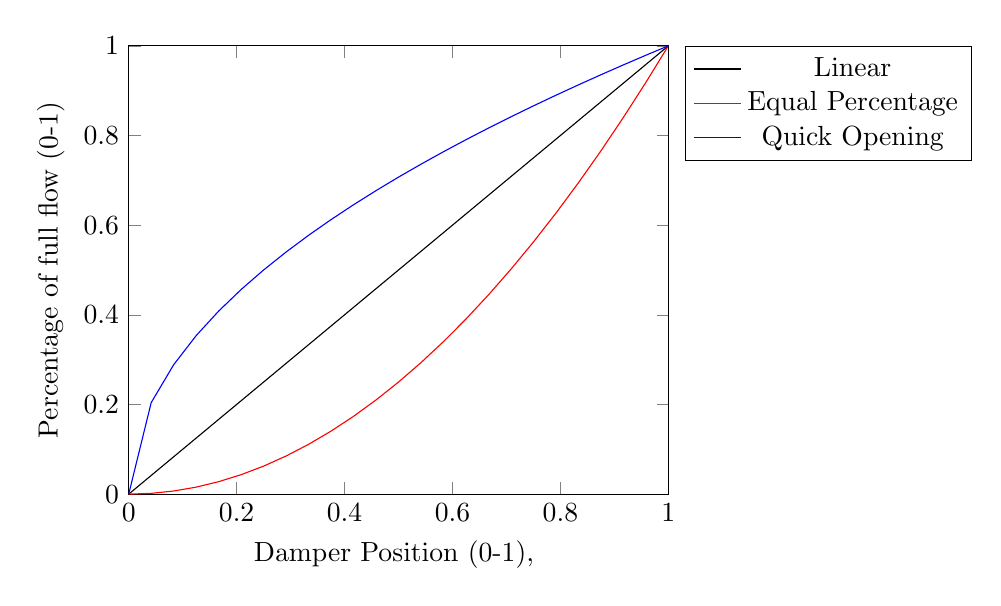
\begin{tikzpicture}

\begin{axis}[
        xmin=0,
        xmax=1,
        ymax=1,
        ymin=0,
        legend pos=outer north east,
        xlabel={Damper Position (0-1), \(\damp{}\)},
        ylabel={Percentage of full flow (0-1)},
    ] \addplot[
        domain=0:1,
        black,
    ]
    {x};

    \addlegendentry{Linear}

    \addplot[
        domain=0:1,
        red,
    ]{x*x};
    \addlegendentry{Equal Percentage}

    \addplot[
        domain=0:1,
        blue,
    ]{sqrt(x)};
    \addlegendentry{Quick Opening}


\end{axis}



\end{tikzpicture}
\caption{Terminal box flow response as a function of damper position.}
\label{fig:flowVersusDamperPos}
\end{figure}


\section{Predicting the Mixed Air Temperature}

In order to predict the energy use at the cooling/reheat coils in the air handling unit, the mixed air temperature needs to be estimated. The mixed air temperature will be dependent on several variables including the outdoor air temperature, return air temperature, and the damper positions of the outdoor air and return air. The damper positions will fluctuate greatly during times of economizing.  


\section{Searching for Energy Minimum}

The fan power can be estimated using a fan curve as a function of the part load ratio (PLR) calculated using air flow rate. A fan curve suggested by Kimla that accounts for VSDs and constant static pressure setpoints is
\begin{equation}\label{eq:KimlaFanPower}
\frac{\dot{W}}{\dot{W}_{rated}} = 0.0013+0.147\left(PLR \right)+0.9506\left(PLR \right)^2-0.0998\left(PLR \right)^3
\end{equation}
where \(PLR\) is defined as \(\frac{\dot{V}}{\dot{V}_{design}}\).

Since we are going to be using the gradient of this function, it is desired to reduce the order to the polynomial from 3 to 2. The corresponding closest second order polynomial to \ref{eq:KimlaFanPower} is
\begin{equation}\label{eq:finalFanPower}
\frac{\dot{W}}{\dot{W}_{rated}} = 0.21\left(PLR \right)+0.8\left(PLR \right)^2
\end{equation}

The total energy is the combination of fan, cooling, and reheat energy. If there are \(n\) terminal units, the total energy can be written as
\begin{multline}\label{eq:totalEnergy}
\energy=\dot{W}_{rated}\;0.8 \left(\frac{\flowsum}{\dot{V}_{design}} \right)^2 + \dot{W}_{rated}\;0.21 \left(\frac{\flowsum}{\dot{V}_{design}} \right)\\
+1.08\left(\flowsum \right)\left(T_{ma}-T_{sa} \right)\\
+1.08\left(V_1 \right)\left(T_{z,1}-\frac{\dot{Q}}{1.08\; V_1} -T_{sa}\right) +1.08\left(V_2 \right)\left(T_{z,2}-\frac{\dot{Q}}{1.08\; V_2} -T_{sa}\right)\\ 
+\ldots+1.08\left(V_n \right)\left(T_{z,n}-\frac{\dot{Q}}{1.08\; V_n} -T_{sa}\right) 
\end{multline}
The first line is related to the fan energy, the second line is related to the cooling load at the air handling unit, and the last two lines relate to reheat energy use. 

This function \ref{eq:totalEnergy} is minimized under the constraints
\begin{align}
V_{min}&\leq V_1, V_2, \ldots V_n \\
T_{sa,min}&\leq T_{sa} \leq T_{sa,max} \\
\sum_i^n V_i &= V_T \leq V_{T,design} \\
\forall i\in\left\{1,\ldots,n\right\}: T_{dis,i} &= T_{z,i} - \frac{\dot{Q}_i}{1.08\;V_i} \geq T_{sa}
\end{align}

The partial derivatives of \ref{eq:totalEnergy} are 
\begin{multline}
\pdv{\dot{E}}{V_i}=\frac{\dot{W}_{design}\;1.6}{\flow{design}^2} \left(\flowsum \right)\\ 
+\frac{0.2\;\dot{W}_{design}}{\dot{V}_{design}}+ 1.08\left(T_{ma}+T_{z,i} -2T_{sa}\right)
\end{multline}
\begin{equation}
\pdv{\dot{E}}{\sat}=-2.16\left(\flowsum \right)
\end{equation}


\begin{figure}
\centering
\begin{tikzpicture}
\begin{axis}[
    xlabel={OA Dry Bulb Temperature (NOAA)},
    ylabel={AHU-1-3 Mixed Air Temp},
]
\addplot[only marks, mark=o]
table[x={OADryBulbTemperature(NOAA)}, y={AHU13MixedAirTemp}, col sep=tab]{Data/2016-05-17-1719-TikzData.dat};
\end{axis}
\end{tikzpicture}
\caption{This is a sample caption.}
\end{figure}






%\begin{sidewaysfigure}
%\begin{tikzpicture}
%
%\coordinate (bottomLeft) at (0,0);
%\coordinate (belowFan) at (0,5); 
%\coordinate (bottomRight) at (10,0);
%\coordinate (topLeft) at (0,13);
%
%\node [circle, draw] at (-2,10) {\(P_{s,fan}\) };
%
%\draw (bottomRight) -- (bottomLeft) -- (belowFan);
%\draw (-0.5,10) -- (0.5,10);
%\draw (-1, 10.5) -- (1,10.5);
%\draw (0,10.5) -- (topLeft);
%
%
%
%
%
%\end{tikzpicture}
%\end{sidewaysfigure}



























